\documentclass[a4paper,10pt]{article}
%\documentclass[a4paper,10pt]{scrartcl}

\usepackage[utf8]{inputenc}
\usepackage{pgf}
\usepackage{tikz}
\usepackage{float}
\usetikzlibrary{arrows}
\usetikzlibrary{automata}
\definecolor{lgrey}{RGB}{190,190,190}
\pdfinfo{%
  /Title    (Assessed Coursework: Systems Verification 303)
  /Author   (Ioannis Kassinopoulos)
  /Creator  (Ioannis Kassinopoulos)
  /Producer (Ioannis Kassinopoulos)
  /Subject  (Systems Verification Coursework)
  /Keywords (verification,coursework,imperial)
}

\begin{document}

\title{Assessed Coursework: Systems Verification}
\author{Ioannis Kassinopoulos}
\date{\today}
\maketitle
\section*{Question 1}
\begin{figure}[H]
  \centering
  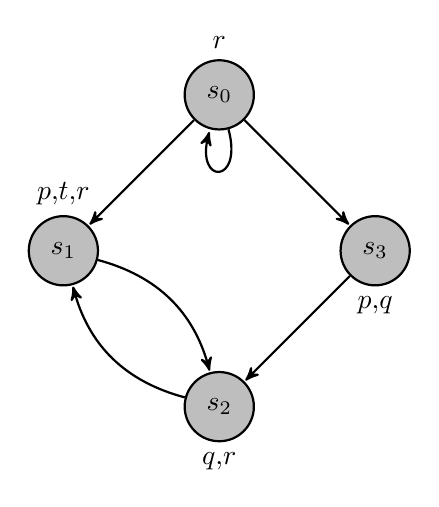
\begin{tikzpicture}[->,>=stealth',shorten >=0.5pt,auto,node distance=2.8cm,thick]
      \tikzstyle{every state}=[fill=lgrey,draw=black,text=black]

      \node[label = above:{$r$},state]		(A) {$s_0$};
      \node[label = above:{$p$,$t$,$r$},state]	(B) [below left of  = A]   {$s_1$};
      \node[label = below:{$p$,$q$},state]	(C) [below right of = A]   {$s_3$};
      \node[label = below:{$q$,$r$},state]	(D) [below right of = B]   {$s_2$};
      
      \path 
	(A) edge			node{} (B)
	(A) edge			node{} (C)
	(A) edge	[loop below]	node{} (A)
	(B) edge	[bend left]	node{} (D)
	(D) edge	[bend left]	node{} (B)
	(C) edge			node{} (D);
      
  \end{tikzpicture}
  \caption{The transition system $\mathcal{M}_1$.}
  \label{fig:m1}
\end{figure}

\subsection*{Algebraic Form}

A transition system $\mathcal{M}=(S,\rightarrow,L)$ is a set of states $S$ endowed with a transition relation 
$\rightarrow$ (a binary relation on $S$), such that every $s \in  S$ has some $s'\in S$ with $s\rightarrow s'$,
and a labeling function $L:S\rightarrow \mathcal{P}$(Atoms).
\\[0.5cm] 
Our system $\mathcal{M}_1$ (figure:~\ref{fig:m1}) can be described as following:
\\[0.cm] 
$\mathcal{P} = \{p,q,r,t\}$
\\[0.10cm] 
$\mathcal{M}_1 = \{\{ s_0,s_1,s_2,s_3 \} , \{ (s_0,s_0),(s_0,s_1),(s_0,s_3),(s_1,s_2),(s_2,s_1),(s_3,s_1)   \} , \pi \}$
\\[0.10cm] 
$\pi(p) = \{s_1,s_3 \}$
\\[0.10cm] 
$\pi(q) = \{s_2,s_3 \}$
\\[0.10cm] 
$\pi(r) = \{s_0,s_1,s_2 \}$
\\[0.10cm] 
$\pi(t) = \{ s_1 \}$
\subsection*{Infinite Tree}
\begin{figure}[H]
  \label{fig:infTree}
  \centering
  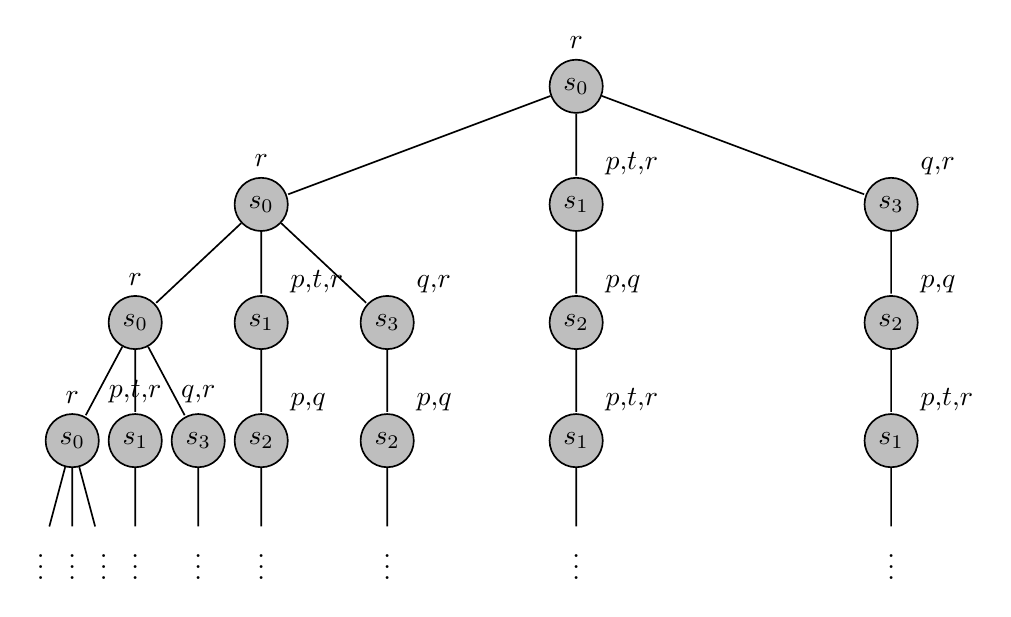
\begin{tikzpicture}[level 2/.style={sibling distance=16mm},level 1/.style={sibling distance=40mm},level 4/.style={sibling distance=4mm},level 3/.style={sibling distance=8mm},level/.style={sibling distance=25mm/#1},-,>=stealth',shorten >=0.5pt,auto,node distance=1cm,semithick]
      \tikzstyle{every state}=[fill=lgrey,draw=black,text=black,inner sep=3pt,minimum size=4pt]
      \node [label = above:{$r$},state] (a){$s_0$}
	child {
	node [label = above:{$r$},state] (b) {$s_0$}
	  child {
	  node [label = above:{$r$},state] (c) {$s_0$}
	    child{
	    node [label = above:{$r$},state] (d) {$s_0$}
	      child{
	      node [] (e) {$\vdots$}
	      }
	      child{
	      node [] (e) {$\vdots$}
	      }
	      child{
	      node [] (e) {$\vdots$}
	      }
	    }
	    child{
	    node [label = above:{$p$,$t$,$r$},state] (d) {$s_1$}
	      child{
	      node [] (e) {$\vdots$}
	      }
	    }
	    child{
	    node [label = above:{$q$,$r$},state] (d) {$s_3$}
	    child{
	      node [] (e) {$\vdots$}
	      }
	    }
	  }
	  child {
	  node [label = above right:{$p$,$t$,$r$},state] (c) {$s_1$}
	    child {
	    node [label = above right:{$p$,$q$},state] (d) {$s_2$}	      
	    child {
	    node [] (e) {$\vdots$}	      
	    }
	    }
	  }	  
	  child {
	    node [label = above right:{$q$,$r$},state] (c) {$s_3$}
	      child {
	      node [label = above right:{$p$,$q$},state] (d) {$s_2$}	      
		child {
		node [] (e) {$\vdots$}	      
	      }
	    }
	  }
	}
	child {
	node [label = above right:{$p$,$t$,$r$},state] (b) {$s_1$}
	  child {
	  node [label = above right:{$p$,$q$},state] (c) {$s_2$}
	    child {
	    node [label = above right:{$p$,$t$,$r$},state] (d) {$s_1$}
	      child {
	      node [] (e) {$\vdots$}	      
	      }
	    }
	  }
	}
	child {
	node [label = above right:{$q$,$r$},state] (b) {$s_3$}
	child {
	node [label = above right:{$p$,$q$},state] (c) {$s_2$}
	  child {
	  node [label = above right:{$p$,$t$,$r$},state] (d) {$s_1$}
	    child {
	    node [] (e) {$\vdots$}
	    }
	  }
	}
	};
  \end{tikzpicture}
  \caption{Unwinding the system described by  $\mathcal{M}_1$ as an infinite tree of all computation paths beginning in $s_0$ (first layer).}
\end{figure}

\subsection*{Satisfiability}


\section*{Question 2}
\section*{Question 3}
\section*{Question 4}


\end{document}
